\section{Initialization choice}
In this project, two different initializations for the weight and bias are used. For the TanH layer, the Xavier initialization is use, thus the weight are initialize from a random distribution with a mean of $0$ and a variance of $\dfrac{2}{size^{Layer-1}+size^{Layer}}$ and initialize the bias to $0$. For the ReLu layer, the He initialization is use which is the same initialization as Xavier initialization but with two time the variance. Those initialization help to reduce the risk that the gradients vanish or explode.

\begin{figure}[H]
	\begin{subfigure}[h]{0.35\textwidth}
		\begin{center}
			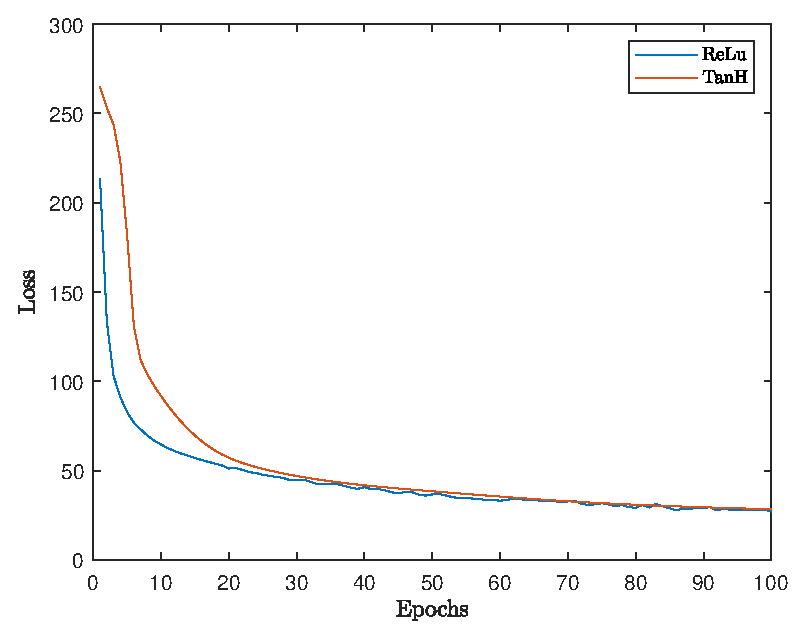
\includegraphics[width=\textwidth]{loss}
		\end{center}
	\end{subfigure}
	\begin{subfigure}[h]{0.35\textwidth}
		\begin{center}
			\includegraphics[width=\textwidth]{accuracy}
		\end{center}
	\end{subfigure}
	\caption{Average of 5 measure of loss and accuracy of the neural network $2$ input and  output and $3$ hidden layer of $25$ neuron each, with the following parameters : $100$ epochs, batch size of $1$, learning rate of $0.02$}
	\label{img::loss_accuracy}
\end{figure}

In Figure ~\ref{img::loss_accuracy}, we can see the result of two neural network with $2$ input, $2$ output and $3$ hidden layer of $25$ neuron each. The blue one is with ReLu layer and the red on is with TanH layer. We can see that the loss converge for the two type of layer. With the chosen parameters, we can see that TanH have better accuracy but is slower to converge than the ReLu layer. The initialization was also test with a variance of $1$, but with this parameter the loss diverge.